\begin{figure}[H]
	\center
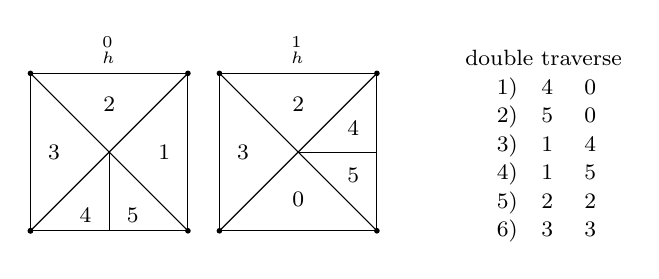
\begin{tikzpicture}[scale=2]
		
		\def \xone{0};
		\def \yone{0};		
		% first rectangle
		\coordinate (A) at (\xone,\yone);
		
        \draw (A) -- ++(0,1) -- ++(1,0)-- ++(0,-1) --cycle;
        \draw (A) -- ++(1,1);
        \draw (A) ++(0,1) -- ++(1,-1);
        \draw (A) ++(0.5,0) -- ++(0,0.5);
        \filldraw (A)         circle (0.4pt);
        \filldraw (A) ++(1,0) circle (0.4pt);
        \filldraw (A) ++(0,1) circle (0.4pt);
        \filldraw (A) ++(1,1) circle (0.4pt);
        
        \fill[black,font=\footnotesize] (A)  ++(0.5,1) node[above] {$\T^0_h$}
        								(A)  ++(0.35,0.1) node	   {$4$}
        								(A)  ++(0.65,0.1) node	   {$5$}
        								(A)  ++(0.15,0.5) node	   {$3$}
        								(A)  ++(0.5,0.8) node	   {$2$}
        								(A)  ++(0.85,0.5) node	   {$1$};
        
        % second rectangle
        \coordinate (A1) at (\xone + 1.2,\yone);
        
        \draw (A1) -- ++(0,1) -- ++(1,0)-- ++(0,-1) --cycle;
        \draw (A1) -- ++(1,1);
        \draw (A1) ++(0,1) -- ++(1,-1);
        \draw (A1) ++(0.5,0.5) -- ++(0.5,0);
        \filldraw (A)         circle (0.4pt);
        \filldraw (A1)         circle (0.4pt);
        \filldraw (A1) ++(1,0) circle (0.4pt);
        \filldraw (A1) ++(0,1) circle (0.4pt);
        \filldraw (A1) ++(1,1) circle (0.4pt);
        
        \fill[black,font=\footnotesize] (A1) ++(0.5,1) node[above] {$\T^1_h$}
        								(A1)  ++(0.85,0.65) node	   {$4$}
        								(A1)  ++(0.85,0.35) node	   {$5$}
        								(A1)  ++(0.15,0.5) node	   {$3$}
        								(A1)  ++(0.5,0.8) node	   {$2$}
        								(A1)  ++(0.5,0.2) node	   {$0$};
        
         % coarse rectangle
%        \coordinate (A2) at (\xone - 1.2,\yone);
        
%        \draw (A2) -- ++(0,1) -- ++(1,0)-- ++(0,-1) --cycle;
%        \draw (A2) -- ++(1,1);
%        \draw (A2) ++(0,1) -- ++(1,-1);
%        \filldraw (A)         circle (0.4pt);
%        \filldraw (A2)         circle (0.4pt);
%        \filldraw (A2) ++(1,0) circle (0.4pt);
%        \filldraw (A2) ++(0,1) circle (0.4pt);
%        \filldraw (A2) ++(1,1) circle (0.4pt);
        
%        \fill[black,font=\footnotesize] (A2) ++(0.5,1) node[above] {coarse}
%        								(A2)  ++(0.5,0.2) node	   {$0$}
%        								(A2)  ++(0.15,0.5) node	   {$3$}
%								        (A2)  ++(0.5,0.8) node	   {$2$}
%        								(A2)  ++(0.85,0.5) node	   {$1$};
        								
        \coordinate (A3) at (\xone + 2.9,\yone);
        \fill[black,font=\footnotesize] (A3) ++(-0.2,1.1) node[right] {double traverse}
        								(A3) ++(0,0.9) 	  node[right] {1)\quad 4 \quad 0}
        								(A3) ++(0,0.72)   node[right] {2)\quad 5 \quad 0}
								        (A3) ++(0,0.54)   node[right] {3)\quad 1 \quad 4}
								        (A3) ++(0,0.36)   node[right] {4)\quad 1 \quad 5}
        								(A3) ++(0,0.18)   node[right] {5)\quad 2 \quad 2}
        								(A3) 			  node[right] {6)\quad 3 \quad 3};
        
\end{tikzpicture}

\caption{double traverse}
\label{ch_mult_traverse}
\end{figure}